
\documentclass[11pt]{article}

\usepackage[margin=1in]{geometry}
\usepackage{amsmath, amssymb}
\usepackage{graphicx}
\usepackage{xcolor}
\usepackage{booktabs}
\usepackage{fancyhdr}
\usepackage{import}
\usepackage{enumitem}
\usepackage{setspace}
\usepackage{longtable}
\usepackage{float} 
\usepackage[compact]{titlesec}
\usepackage{caption}
\usepackage{listings}
\usepackage{tikz}
\usetikzlibrary{shapes.geometric, shapes.misc, arrows.meta, positioning, fit, backgrounds, calc}
\usepackage{xcolor}
\captionsetup[table]{position=above}
\setstretch{1.2}
\usepackage[backend=biber,style=apa]{biblatex}
\addbibresource{references.bib}

\newcommand{\question}[1]{\noindent\hspace{2em}\textbf{#1}}

\pagestyle{fancy}
\geometry{a4paper, margin=2.3cm}

\fancyhf{}

% Header
\fancyhead[L]{\small EGH490  }
\fancyhead[C]{\small QUT Microgrid Telemetry System}
\fancyhead[R]{\small Dylan Hessing}

% Footer
\fancyfoot[L]{\small Faculty of Engineering}
\fancyfoot[C]{\small\thepage}
\fancyfoot[R]{\small\today}

% Line thickness
\renewcommand{\headrulewidth}{0.4pt}
\renewcommand{\footrulewidth}{0.4pt}
% Define QUT blue
\definecolor{qutblue}{RGB}{0, 92, 169}
\definecolor{darkblue}{HTML}{1E3A5F}
\definecolor{influxorange}{HTML}{D94C2B}
\definecolor{codebg}{HTML}{F5F5F5}
\definecolor{codefg}{HTML}{2D2D2D}
\definecolor{commentgrey}{HTML}{6A6A6A}
\definecolor{delim}{RGB}{20,105,176}
\definecolor{numb}{RGB}{106, 109, 32}
\definecolor{string}{rgb}{0.64,0.08,0.08}

\lstdefinelanguage{json}{
    numbers=left,
    numberstyle=\small,
    frame=single,
    rulecolor=\color{black},
    showspaces=false,
    showtabs=false,
    breaklines=true,
    postbreak=\raisebox{0ex}[0ex][0ex]{\ensuremath{\color{gray}\hookrightarrow\space}},
    breakatwhitespace=true,
    basicstyle=\ttfamily\small,
    upquote=true,
    morestring=[b]",
    stringstyle=\color{string},
    literate=
     *{0}{{{\color{numb}0}}}{1}
      {1}{{{\color{numb}1}}}{1}
      {2}{{{\color{numb}2}}}{1}
      {3}{{{\color{numb}3}}}{1}
      {4}{{{\color{numb}4}}}{1}
      {5}{{{\color{numb}5}}}{1}
      {6}{{{\color{numb}6}}}{1}
      {7}{{{\color{numb}7}}}{1}
      {8}{{{\color{numb}8}}}{1}
      {9}{{{\color{numb}9}}}{1}
      {\{}{{{\color{delim}{\{}}}}{1}
      {\}}{{{\color{delim}{\}}}}}{1}
      {[}{{{\color{delim}{[}}}}{1}
      {]}{{{\color{delim}{]}}}}{1},
}


\lstdefinelanguage{toml}{
    morekeywords={true,false},
    morecomment=[l]{\#},
    morestring=[b]",
    morestring=[b]',
    keywordstyle=\color{blue},
    commentstyle=\color{gray},
    stringstyle=\color{orange},
    basicstyle=\ttfamily\small,
    breaklines=true,
}

\lstset{
  backgroundcolor=\color{codebg},
  basicstyle=\ttfamily\small\color{codefg},
  breaklines=true,
  frame=single,
  framerule=0pt,
  rulecolor=\color{codebg},
  xleftmargin=8pt,
  xrightmargin=8pt,
  aboveskip=8pt,
  belowskip=8pt,
  showstringspaces=false,
}
\lstdefinelanguage{Flux}{
  morekeywords={from, range, filter, group, map, yield, sum, count, mean},
  sensitive=true,
  morecomment=[l]{//},
  morestring=[b]",
  alsoletter={>},
  morekeywords=[2]{|>}, % Pipe forward operator
  keywordstyle=[2]\color{blue}\bfseries,
}

% ── Colour palette (QUT blue + neutral greys) ──────────────────────────────
\definecolor{qutblue}{RGB}{0, 60, 113}
\definecolor{nodebg}{RGB}{220, 232, 245}
\definecolor{serverbg}{RGB}{240, 245, 250}
\definecolor{arrowcol}{RGB}{80, 80, 80}
\definecolor{groupborder}{RGB}{160, 185, 210}
\definecolor{labelgrey}{RGB}{90, 90, 90}

\tikzset{
  % Hardware DAQ node boxes
  daqnode/.style={
    rectangle, rounded corners=4pt,
    draw=qutblue, line width=1.2pt,
    fill=nodebg,
    minimum width=3.2cm, minimum height=1.0cm,
    font=\sffamily\small, text centered,
    inner sep=6pt
  },
  % Software component boxes on historian server
  swbox/.style={
    rectangle, rounded corners=4pt,
    draw=qutblue, line width=1.2pt,
    fill=white,
    minimum width=3.0cm, minimum height=0.9cm,
    font=\sffamily\small, text centered,
    inner sep=6pt
  },
  % Storage / database component
  dbbox/.style={
    cylinder, shape border rotate=90,
    draw=qutblue, line width=1.2pt,
    fill=white,
    minimum width=2.8cm, minimum height=1.0cm,
    font=\sffamily\small, text centered,
    inner sep=4pt,
    aspect=0.25
  },
  % Small annotation label
  annot/.style={
    font=\sffamily\scriptsize\itshape,
    text=labelgrey
  },
  % Protocol label on arrows
  proto/.style={
    font=\sffamily\scriptsize,
    fill=white, inner sep=2pt,
    text=qutblue
  },
  % Arrow style
  myarrow/.style={
    -{Latex[length=2.5mm, width=2mm]},
    line width=1.0pt,
    color=arrowcol
  },
  % Dashed boundary box label
  grouplabel/.style={
    font=\sffamily\footnotesize\bfseries,
    text=qutblue
  }
}

\setlength{\parindent}{0pt}
\setlength{\parskip}{1em}


\usepackage{fontspec}
\setmainfont{Carlito} 


\title{Literature Review}

\author{Dylan Hessing}
\begin{document}

\begin{titlepage}
    \centering

    % Logo at top
    
\includegraphics[width=0.35\textwidth]{QUT.jpg}\par
    \vspace{0.3cm}
    
    % Faculty and unit
    {\large\color{qutblue}\textbf{Faculty of Engineering}\par}
    {\normalsize Internal Design Document\par}
    
    \vspace{0.8cm}
    \textcolor{qutblue}{\rule{\linewidth}{1mm}}\par
    \vspace{0.5cm}

    % Title
    {\LARGE\bfseries InfluxDB Design for Distributed\\[0.3em]
    Real-Time Telemetry System for QUT Microgrid\par}
    \vspace{0.3cm}

    \vspace{0.5cm}
    \textcolor{qutblue}{\rule{\linewidth}{1mm}}\par
    \vspace{0.8cm}

    % Info table
    \begin{tabular}{@{}ll@{}}
        \textbf{Date:}             & \today                    \\[0.5em]
        \textbf{Student Engineer:} & Dylan Hessing             \\[0.5em]
        \textbf{Student ID:}       & n11245310                 \\[0.5em]
        \textbf{Supervisor:}       & Assoc.\ Prof.\ Geoff Walker \\
    \end{tabular}

    \vfill

    % Version history table
    {\small\textbf{Version History}\par}
    \vspace{0.3cm}
    \begin{tabular}{|c|l|l|l|}
        \hline
        \textbf{Version} & \textbf{Date} & \textbf{Author} & \textbf{Changes / Comments} \\
        \hline
        1 & April 21, 2026 & Dylan Hessing & Initial Design \\
        \hline
        2 & \today & Dylan Hessing & \\
        \hline
    \end{tabular}

\end{titlepage}
\begin{spacing}{1.15}
\tableofcontents
\end{spacing}
\newpage
\section{Overview}
This document describes the design of the InfluxDB historian comnponent within the distributed microgrid telemetry system. The historian is responsible for receiving time--series electrical measurements from time series electrical measurements from distributed DAQ nodes, persisting with nanosecond--precision timestamps derived from PTP--synchronised STM32 firmware and exposing them for downstream query and analysis. 


\section{Scope}
This document assumes the MQTT protocol design described in the companision document MQTT Protocol Design for Distributed Real-Time Telemetry System for QUT Microgrid (April 2026). In particular, it assumes: 
\begin{itemize}[noitemsep]
  \item Mosquitto as the broker 
  \item telegraf as the historian bridge  
  \item The four--level topic hierachy \texttt{microgrid/<node\_id>/<subsystem>/<measurement>},
  \item the JSON payloads carrying a  \texttt{ts} and \texttt{v} field.
\end{itemize}

Hardware design, DAQ node fabrication and RTOS/firmware decisions are out of scope. 



\section{Architecture Overview}

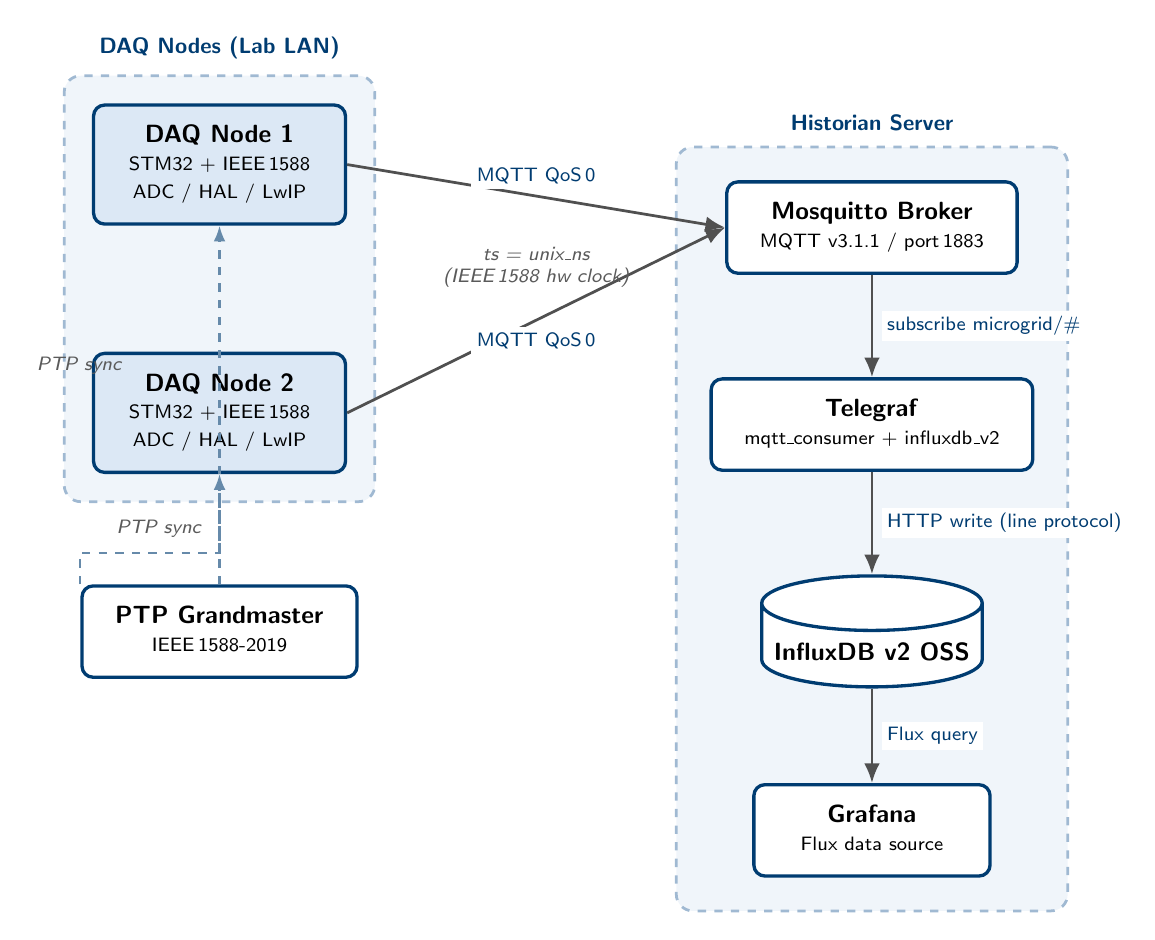
\begin{tikzpicture}[node distance=1.4cm]
 
% ═══════════════════════════════════════════════════════════════════
% DAQ NODES (left column)
% ═══════════════════════════════════════════════════════════════════
 
\node[daqnode] (node1) {%
  \begin{tabular}{c}
    \textbf{DAQ Node 1}\\[-1pt]
    \scriptsize STM32 + IEEE\,1588\\[-1pt]
    \scriptsize ADC / HAL / LwIP
  \end{tabular}};
 
\node[daqnode, below=1.6cm of node1] (node2) {%
  \begin{tabular}{c}
    \textbf{DAQ Node 2}\\[-1pt]
    \scriptsize STM32 + IEEE\,1588\\[-1pt]
    \scriptsize ADC / HAL / LwIP
  \end{tabular}};
 
% ═══════════════════════════════════════════════════════════════════
% PTP GRANDMASTER (below DAQ nodes, centred)
% ═══════════════════════════════════════════════════════════════════
 
\node[swbox, below=1.4cm of node2, xshift=0cm,
      minimum width=3.2cm] (ptp) {%
  \begin{tabular}{c}
    \textbf{PTP Grandmaster}\\[-1pt]
    \scriptsize IEEE\,1588-2019
  \end{tabular}};
 
% ═══════════════════════════════════════════════════════════════════
% HISTORIAN SERVER (right side)
% ═══════════════════════════════════════════════════════════════════
 
% Mosquitto broker
\node[swbox, right=4.8cm of node1, yshift=-0.8cm] (mosquitto) {%
  \begin{tabular}{c}
    \textbf{Mosquitto Broker}\\[-1pt]
    \scriptsize MQTT v3.1.1 / port\,1883
  \end{tabular}};
 
% Telegraf bridge (below Mosquitto)
\node[swbox, below=1.3cm of mosquitto] (telegraf) {%
  \begin{tabular}{c}
    \textbf{Telegraf}\\[-1pt]
    \scriptsize mqtt\_consumer + influxdb\_v2
  \end{tabular}};
 
% InfluxDB (below Telegraf)
\node[dbbox, below=1.3cm of telegraf] (influxdb) {\textbf{InfluxDB v2 OSS}};
 
% Grafana (below InfluxDB)
\node[swbox, below=1.2cm of influxdb] (grafana) {%
  \begin{tabular}{c}
    \textbf{Grafana}\\[-1pt]
    \scriptsize Flux data source
  \end{tabular}};
 
% ═══════════════════════════════════════════════════════════════════
% GROUP BOXES
% ═══════════════════════════════════════════════════════════════════
 
% DAQ nodes boundary
\begin{scope}[on background layer]
  \node[draw=groupborder, dashed, line width=1pt,
        fill=serverbg, rounded corners=6pt,
        fit=(node1)(node2),
        inner sep=10pt] (daqgroup) {};
\end{scope}
\node[grouplabel, above=2pt of daqgroup.north] {DAQ Nodes (Lab LAN)};
 
% Historian server boundary
\begin{scope}[on background layer]
  \node[draw=groupborder, dashed, line width=1pt,
        fill=serverbg, rounded corners=6pt,
        fit=(mosquitto)(telegraf)(influxdb)(grafana),
        inner sep=12pt] (servergroup) {};
\end{scope}
\node[grouplabel, above=2pt of servergroup.north] {Historian Server};
 
% ═══════════════════════════════════════════════════════════════════
% ARROWS
% ═══════════════════════════════════════════════════════════════════
 
% Node 1 → Mosquitto  (MQTT publish)
\draw[myarrow] (node1.east) -- (mosquitto.west)
  node[proto, midway, above=2pt] {MQTT QoS\,0};
 
% Node 2 → Mosquitto
\draw[myarrow] (node2.east) -- (mosquitto.west)
  node[proto, midway, below=2pt] {MQTT QoS\,0};
 
% Mosquitto → Telegraf (internal subscription)
\draw[myarrow] (mosquitto.south) -- (telegraf.north)
  node[proto, midway, right=3pt] {subscribe microgrid/\#};
 
% Telegraf → InfluxDB (line protocol write)
\draw[myarrow] (telegraf.south) -- (influxdb.north)
  node[proto, midway, right=3pt] {HTTP write (line protocol)};
 
% InfluxDB → Grafana (Flux query)
\draw[myarrow] (influxdb.south) -- (grafana.north)
  node[proto, midway, right=3pt] {Flux query};
 
% PTP sync arrows (dashed, bidirectional)
\draw[-{Latex[length=2mm]}, dashed, line width=0.8pt, color=qutblue!60]
  (ptp.north) -- (node2.south)
  node[annot, midway, left=3pt] {PTP sync};
 
\draw[-{Latex[length=2mm]}, dashed, line width=0.8pt, color=qutblue!60]
  (ptp.north west) -- ++(0,0.4) -| (node1.south)
  node[annot, near start, left=3pt] {};
 
% PTP label on node1 line
\node[annot] at ($(node1.south)!0.5!(ptp.north west) + (-0.9,0.5)$) {PTP sync};
 
% ═══════════════════════════════════════════════════════════════════
% TIMESTAMP ANNOTATION
% ═══════════════════════════════════════════════════════════════════
\node[annot, align=center, text width=3.5cm]
  at ($(node1.east)!0.5!(mosquitto.west) + (0,-0.9)$)
  {ts = unix\_ns\\(IEEE\,1588 hw clock)};
 
\end{tikzpicture}

Mosquitto and InfluxDB are co-deployed on the same historian server, consistent with the MQTT design's broker configuration. Telegraf runs on the same server host as the intermediary bridge (no custom subscriber code is required).

\section{InfluxDB Version Selection}
InfluxDB v2 OSS is selected as the historian for this project. The justification centres on four properties that are directly required by the system design.

Flux query language and native task scheduling. InfluxDB v2 is the only version for which Flux is the primary, fully--supported query interface, and all dashboard and analysis queries are written in Flux. The original downsampling design relied on Flux scheduled tasks running within the database; as built, downsampling is performed by the ingestion service instead (Section~\ref{sec:downsampling}), but the integrated task scheduler remains available without an external Kapacitor instance, keeping the Docker Compose stack minimal and operationally simple, appropriate for a single--historian research testbed.

Telegraf influxdb\_v2 output plugin and HTTP write API. The JSON ingestion path is entirely configuration--driven via Telegraf's mqtt\_consumer input and influxdb\_v2 output plugin. This plugin (including the \texttt{json\_time\_key} and \texttt{json\_time\_format = "unix\_ns"} features central to this design) is a first--class, mature integration with InfluxDB v2, with extensive documentation and community usage. The full-rate path writes batched, gzip-compressed line protocol directly to the same v2 HTTP API (Section~\ref{sec:fullrate}).

Token-based access control. InfluxDB v2's token--based authentication model supports bucket--scoped write tokens, which is the basis of the planned security posture (Section~\ref{sec:security}): write-only tokens scoped to their buckets for Telegraf and \texttt{daq2-ingest}, and a separate read-only token for Grafana. This fine-grained token model is native to v2, although the scoped tokens have not yet been issued.

Grafana Flux data source. Grafana's native Flux data source for InfluxDB v2 is stable and well--supported, enabling the dashboard panels (Section~\ref{sec:grafana}) to query the historian directly in Flux.

Relationship to InfluxDB 3 Core. InfluxDB 3 Core reached general availability in April 2025.  However, InfluxDB 3 Core is not positioned as a direct replacement for InfluxDB OSS v2, and v2 is not planned to reach end--of--life. The v3 architecture is a significant departure — it replaces Flux with native SQL and InfluxQL, and integrates a Python processing engine in place of the Kapacitor/task model used in v2.  Migrating to v3 would require rewriting all Flux queries documented here and the provisioned dashboard, with no clear benefit at this testbed scale. InfluxDB v2 OSS therefore remains the appropriate and supported choice for a new deployment of this scope.

Docker image pinning note: The latest tag for InfluxDB Docker images will point to InfluxDB 3 Core from late May 2026 onward.  The Compose file (Section~\ref{sec:compose}) uses the explicit influxdb:2 tag to prevent an unintended upgrade during the thesis validation period. This must not be changed to latest.

\section{Schema \& Data Model}
InfluxDB organises data as:
\begin{center}
Organisation --> bucket --> Measurement --> Tags + Field + Timestamp
\end{center}

\subsection{Organisation}
A single InfluxDB organisation \texttt{qut-microgrid} is used, consistent with the Telegraf output configuration in the MQTT design document.

\subsection{Buckets}

\begin{table}[H]
  \caption{Buckets}
  \begin{center}
    \begin{tabular}{lll}
      \hline
      \textbf{Bucket} & \textbf{Purpose} & \textbf{Retention} \\
      \hline
      \texttt{telemetry} & Full--resolution samples from all nodes & 90 days (TBD) \\
      \texttt{telemetry\_1m} & 1--minute aggregates for long-term storage & Indefinite \\
      \hline
    \end{tabular}
  \end{center}
\end{table}

The bucket name \texttt{telemetry} matches the Telegraf output configuration. A seperate downsampled bucket avoids data retention growth while preserving long--term trend visibility. 
      
\subsection{Measurements}
Each MQTT subsystem segment maps to a distinct InfluxDB measurement name:

\begin{table}[H]
  \caption{Measuremnts}
  \begin{center}
    \begin{tabular}{ll}
      \hline
      \textbf{Measurement} & \textbf{Description}\\
      \hline
      \texttt{voltage} & Phase voltage samples (V) \\
      \texttt{current} & Phase and neutral current samples (A) \\
      \texttt{status} & Node liveness and heartbeat dignostics \\
      \texttt{ptp\_status} & PTP synchronisation diagnostics \\
      \hline
    \end{tabular}
  \end{center}
\end{table}

Additional subsystems may be introduced without structural schema changes if the STM32 firmware is extended to publish derived quantities.

\subsection{Tags}
Tags are string--valued, indexed, and low--cardinality. All three tags are populated automatically by Telegraf's \texttt{topic\_parsing} from the four--level MQTT topic hierachy. 

\begin{table}[H]
  \caption{Tags}
  \begin{center}
    \begin{tabular}{llp{0.2\linewidth}p{0.4\linewidth}}
      \hline
      \textbf{Tag Key} & \textbf{Source} & \textbf{Example Values} & \textbf{Notes}\\
      \hline
      \texttt{node\_id} & Topic segment 2 & \texttt{node\_1}, \texttt{node\_2} & Fixed at firmware flash time, MAC/IP addresses explicitly avoided. \\
      \texttt{measurement} & Topic segment 4 & \texttt{va}, \texttt{ib} & Aligned with IEEE-1459-2010 notation \\
      \hline
    \end{tabular}
  \end{center}
\end{table}

\subsection{Fields}
\begin{table}[H]
  \caption{Tags}
  \begin{center}
    \begin{tabular}{lllp{0.5\linewidth}}
      \hline
      \textbf{Field Key} & \textbf{Type} & \textbf{Source} & \textbf{Units}\\
      \hline
      \texttt{v} & float64 & JSON payload \texttt{v} field & implied by \texttt{\_measurement} and \texttt{measurement} tag (V or A) \\
      \hline
    \end{tabular}
  \end{center}
\end{table}

\subsection{Timestamp}
Timestamps are written at nanosecond precision using the \texttt{ts} field from the JSON payload, sourced from the STM32 IEEE 1588 hardware timestamping peripheral. The historian does not substitute broker receive time or Telegraf processing time: the node--reported PTP timestamp is authoritative end--to--end.

\subsection{Representative Schema}
\begin{table}[H]
  \caption{Representative Schema}
  \begin{center}
    \begin{tabular}{lllll}
      \hline
      \textbf{subsystem (\_measurement)} & \textbf{node\_id} & \textbf{measurement} & \textbf{\_field} & \textbf{Example Value}\\
      \hline
      \texttt{voltage} & \texttt{node\_1} & \texttt{va} & \texttt{v} & \\
      \texttt{voltage} & \texttt{node\_1} & \texttt{vb} & \texttt{v} & \\
      \texttt{voltage} & \texttt{node\_1} & \texttt{vc} & \texttt{v} & \\
      \texttt{current} & \texttt{node\_1} & \texttt{ia} & \texttt{v} & \\
      \texttt{current} & \texttt{node\_1} & \texttt{ib} & \texttt{v} & \\
      \texttt{current} & \texttt{node\_1} & \texttt{ic} & \texttt{v} & \\
      \texttt{ptp\_status} & \texttt{node\_1} & \texttt{offset\_ns} & \texttt{v} & \\
      \hline
    \end{tabular}
  \end{center}
\end{table}








\section{Ingestion Pipeline}
\label{sec:ingestion}

\subsection{Overview}
This section describes the low-rate JSON path (\texttt{microgrid/\#}), which is fully configuration-driven via Telegraf's MQTT consumer input plugin, regex and Starlark processors, and the InfluxDB v2 output plugin, with no custom code. Telegraf runs as a Docker container on the historian server alongside Mosquitto and InfluxDB. The full-rate binary stream is ingested by a separate service (Section~\ref{sec:fullrate}).

\subsection{Telegraf Configuration}
The as-built configuration (\path{telegraf/telegraf.conf}) is:
\begin{lstlisting}[language=toml]
[agent]
  interval = "10s"
  flush_interval = "1s"
  precision = "1ns"
  omit_hostname = true

[[inputs.mqtt_consumer]]
  servers = ["tcp://mosquitto:1883"]
  topics = ["microgrid/#"]
  qos = 0
  data_format = "json"
  json_time_key = "ts"
  json_time_format = "unix_ns"
  topic_tag = "topic"

[[processors.regex]]
  order = 1
  [[processors.regex.tags]]
    key = "topic"
    pattern = "^microgrid/([^/]+)/([^/]+)/([^/]+)$"
    replacement = "${1}"
    result_key = "node_id"
  # ... likewise ${2} -> subsystem, ${3} -> metric

[[outputs.influxdb_v2]]
  urls = ["http://influxdb:8086"]
  token = "${INFLUXDB_TOKEN}"
  organization = "qut-microgrid"
  bucket = "telemetry"
\end{lstlisting}
Notes:
\begin{itemize}[noitemsep]
  \item \texttt{json\_time\_key = "ts"} and \texttt{json\_time\_format = "unix\_ns"} make Telegraf use the node's PTP-derived timestamp as the InfluxDB point timestamp verbatim, and \texttt{precision = "1ns"} preserves its full resolution.
  \item The full topic is kept as the \texttt{topic} tag, and the regex processor extracts \texttt{node\_id}, \texttt{subsystem}, and \texttt{metric} from it. This replaced the \texttt{topic\_parsing} block of the original design.
  \item Telegraf reaches the broker and database by container name over the internal Docker network.
  \item The InfluxDB token is injected via an environment variable and is never stored in the configuration file. The broker requires no credentials (see the MQTT design document).
\end{itemize}

\subsection{Burst Payload Path}
Each JSON burst \texttt{\{"ts", "sync", "dt\_ns", "v": [20 values]\}} is parsed into a single point: Telegraf's JSON parser flattens the \texttt{v} array into fields \texttt{v\_0} to \texttt{v\_19}, and \texttt{sync} and \texttt{dt\_ns} become numeric fields. The parser cannot reconstruct per-sample timestamps itself. Booleans and strings are dropped by the parser, which is why the firmware sends \texttt{sync} as an integer.

\paragraph{Burst Splitting} A Starlark processor, run after the regex processor, splits each burst into individually timestamped points. For every burst point it emits 20 additional points in the \texttt{samples} measurement, sample $k$ at \texttt{ts} $+ k \cdot$ \texttt{dt\_ns}, carrying the burst's tags and the fields \texttt{v} and \texttt{sync}:

\begin{lstlisting}[language=toml]
[[processors.starlark]]
  order = 2
  source = '''
def apply(metric):
    if "dt_ns" not in metric.fields or "v_0" not in metric.fields:
        return metric
    dt = int(metric.fields["dt_ns"])
    sync = metric.fields.get("sync")
    out = [metric]
    for k in range(1024):
        key = "v_" + str(k)
        if key not in metric.fields:
            break
        sample = Metric("samples")
        for name, value in metric.tags.items():
            sample.tags[name] = value
        sample.fields["v"] = metric.fields[key]
        if sync != None:
            sample.fields["sync"] = sync
        sample.time = metric.time + k * dt
        out.append(sample)
    return out
'''
\end{lstlisting}

The original burst point is retained alongside the samples, so that existing dashboards and the liveness check are unaffected; at the JSON path's rate the duplication is negligible. This path is the low-rate fallback for when the full-rate stream is not in use. The full-rate binary stream on \texttt{daq2/<node\_id>/samples} lies outside Telegraf's subscribed topic tree and is ingested separately (Section~\ref{sec:fullrate}).

\subsection{Write Batching}
\begin{table}[H]
  \caption{Write Batching}
  \begin{center}
    \begin{tabular}{lll}
      \hline
      \textbf{Parameter} & \textbf{Value} & \textbf{Notes} \\
      \hline
      \texttt{metric\_batch\_size} & 1000 points (default) & Maximum points per write request \\
      \texttt{flush\_interval} & 1s & Maximum time between flushes \\
      \hline
    \end{tabular}
  \end{center}
\end{table}
At the as-built publish rate (six bursts per node every 5~s, plus one PTP status message per second) the write load is small. The 1~s flush interval keeps PTP status as current as the Node View dashboard, which refreshes every second.

\subsection{QoS Alignment}
Telemetry is published at QoS~0, consistent with the MQTT design. The ingestion pipeline makes no attempt to detect or fill gaps in the historian record resulting from dropped packets or node disconnection. Gaps are visible in the historian and are acceptable for a research testbed.

\subsection{Error Handling}
Telegraf drops malformed payloads that fail JSON parsing and logs an error. No dead-letter queue is implemented. This is acceptable given:
\begin{itemize}[noitemsep]
  \item the two-node testbed operates on a wired LAN with low packet loss probability,
  \item telemetry is QoS~0 by design, so loss is already tolerated at the transport layer, and
  \item a dead-letter mechanism would add operational complexity disproportionate to the research context.
\end{itemize}

\section{Query \& Retention Policies}
\subsection{Retention Design}
Retention is configured at the bucket level in InfluxDB v2. No retention policy is applied within a bucket; the bucket-level setting is the sole retention mechanism.

\begin{table}[H]
  \caption{Measuremnts}
  \begin{center}
    \begin{tabular}{lll}
      \hline
      \textbf{Bucket} & \textbf{Telemetry} & \textbf{Rationale}\\
      \hline
      \texttt{telemetry} & 90 days & Covers the active thesis validation period at full resolution \\
      \texttt{telemetry\_1m} & Indefinite & Long--term aggregate data for reporting and trend analysis \\
      \hline
    \end{tabular}
  \end{center}
\end{table}

\subsection{Downsampling Task}
A Flux scheduled task aggregates telemetry into telemetry\_1m at 1--minute intervals. mean, min, and max are stored as separate fields to support both trend analysis and power quality event detection within each window.

\begin{lstlisting}[language=flux]
option task = {name: "downsample_1m", every: 1m}

from(bucket: "telemetry")
  |> range(start: -task.lastSuccessTime)
  |> filter(fn: (r) => r._field == "v")
  |> aggregateWindow(every: 1m, fn: mean, createEmpty: false)
  |> set(key: "_field", value: "v_mean")
  |> to(bucket: "telemetry_1m")

from(bucket: "telemetry")
  |> range(start: -task.lastSuccessTime)
  |> filter(fn: (r) => r._field == "v")
  |> aggregateWindow(every: 1m, fn: min, createEmpty: false)
  |> set(key: "_field", value: "v_min")
  |> to(bucket: "telemetry_1m")

from(bucket: "telemetry")
  |> range(start: -task.lastSuccessTime)
  |> filter(fn: (r) => r._field == "v")
  |> aggregateWindow(every: 1m, fn: max, createEmpty: false)
  |> set(key: "_field", value: "v_max")
  |> to(bucket: "telemetry_1m")
\end{lstlisting}

\subsection{Key Query Parameters}
The following Flux examples cover the primary query patterns anticipated during validation.

Time-window data for a single channel:
\begin{lstlisting}[language=flux]
from(bucket: "telemetry")
  |> range(start: -1h)
  |> filter(fn: (r) => r._measurement == "voltage"
                    and r.node_id == "node_1"
                    and r.measurement == "va")
\end{lstlisting}

Cross-node comparison for the same channel:
\begin{lstlisting}[language=flux]
from(bucket: "telemetry")
  |> range(start: -1h)
  |> filter(fn: (r) => r._measurement == "voltage"
                    and r.measurement == "va")
  |> group(columns: ["node_id"])
\end{lstlisting}

Cross--node comparisons are only meaningful where PTP synchronisation is confirmed locked. The ptp\_status measurement should be checked before drawing cross--node conclusions from the historian.

All channels from a single node (debugging):
\begin{lstlisting}[language=flux]
from(bucket: "telemetry")
  |> range(start: -15m)
  |> filter(fn: (r) => r.node_id == "node_1")
\end{lstlisting}


PTP synchronisation quality over a window:
\begin{lstlisting}[language=flux]
from(bucket: "telemetry")
  |> range(start: -1h)
  |> filter(fn: (r) => r._measurement == "ptp_status"
                    and r.node_id == "node_1")
\end{lstlisting}

\subsection{Grafana Integration}
Grafana is a confirmed thesis deliverable. Grafana connects to InfluxDB v2 via the native Flux data source. Key dashboard panels anticipated:

\begin{table}[H]
  \caption{Measuremnts}
  \begin{center}
    \begin{tabular}{lll}
      \hline
      \textbf{Panel} & \textbf{Source Bucket} & \textbf{Query Pattern}\\
      \hline
      Per--phase voltage time--series & telemetry & Single--Channel, cross--node \\
      Per--phase current time--series & telemetry & Single--Channel, cross--node \\
      PTP offset over time (per node) & telemetry & ptp\_status measurement \\
      1--minute voltage mean/min/max & telemetry\_1m & Single--Channel, cross--node \\
      \hline
    \end{tabular}
  \end{center}
\end{table}
Grafana dashboard design is out of scope for this document and will be addressed in a separate deliverable.


\section{PTP Timestamping Integration}
\subsection{Timestamp Authority}
The STM32 nodes are the authoritative timestamp source. Each node disciplines its local clock to the PTP grandmaster using hardware timestamping in the Ethernet peripheral. The \texttt{ts} field of each burst is the time of its first sample, computed in firmware from a hardware timer that shares the PTP clock's 100~MHz source, at the centre of that sample's accumulated ADC burst; it is not broker receive time or Telegraf processing time.

Telegraf's \texttt{json\_time\_key} and \texttt{json\_time\_format = "unix\_ns"} configuration ensures this timestamp is used as the InfluxDB timestamp verbatim.

\subsection{Timescale}
PTP time is TAI. The firmware converts it to UTC by subtracting a fixed 37~s offset before publishing, as it does not yet parse the UTC offset advertised in the grandmaster's Announce messages. A future leap second would therefore require a firmware update. Before the servo first locks, the node's clock counts from boot; such early bursts carry \texttt{sync} = 0.

\subsection{Clock Domain Consistency}
All nodes share a single PTP clock domain. The historian server's system clock must be on UTC, synchronised to the same grandmaster or to a sufficiently accurate NTP source, so that Flux query time ranges expressed in wall-clock time correspond correctly to stored point timestamps.

\subsection{Out-of-Order Writes}
MQTT QoS 0 with no ordering guarantees means Telegraf may deliver points to InfluxDB with timestamps older than recently written points. InfluxDB handles out-of-order writes within a shard natively. Default shard duration in InfluxDB v2 is one week; behaviour at shard boundaries should be verified if a node reconnects after an outage longer than one week, though this is unlikely in a lab testbed context.

\subsection{PTP Status Logging}
Each burst carries a \texttt{sync} field, set to 1 when the node's PTP servo was locked at capture. The servo reports lock after eight consecutive offsets within 1~\textmu s of the grandmaster, with a Sync message received within the last 3~s. Bursts are only started on data whose timestamp is valid (no clock step or rate change during capture), and are restarted if a clock step occurs mid-collection.

\paragraph{Deferred} The original design published PTP diagnostics (\texttt{offset\_ns}, \texttt{path\_delay\_ns}, and \texttt{sync\_state} with LOCKED, ACQUIRING, and HOLDOVER states) to a separate \texttt{ptp\_status} subsystem. This was replaced by the per-burst \texttt{sync} field. The servo offset and path delay are printed on each node's debug UART but not published, so the historian cannot provide post-hoc offset traces.

\subsection{Timestamp Quality Validation}
Before cross-node comparisons are drawn from the historian, \texttt{sync} should be confirmed as 1 for all nodes across the relevant time window. Alignment between nodes can be measured independently of the historian by comparing the 1 pulse-per-second outputs of the nodes on an oscilloscope. This validation is a prerequisite for any result that relies on cross-node temporal alignment.

\section{Security}

\subsection{Posture}

The historian operates on a university research lab LAN and is not exposed to the public internet. The security design is therefore pragmatic and aligned with the phased approach documented in the companion MQTT design document (\S7.3). This section describes historian-side measures only; broker-side authentication, ACLs, and TLS are covered in the MQTT design document.

\subsection{InfluxDB Access Control}

InfluxDB v2 uses token-based authentication for all API access. Two tokens are issued:

\begin{table}[H]
\centering
\caption{InfluxDB API Tokens}
\begin{tabular}{lll}
\hline
\textbf{Token} & \textbf{Scope} & \textbf{Used by} \\
\hline
Telegraf write token & Write--only to \texttt{telemetry} bucket & Telegraf bridge \\
Admin token          & Full organisation access               & Local admin / ad--hoc Flux queries \\
\hline
\end{tabular}
\end{table}

The Telegraf write token is scoped to the minimum required permission: write access to the \texttt{telemetry} bucket only. It cannot read data, access other buckets, or modify organisation configuration. This limits the blast radius if the token is compromised.

Tokens are stored as environment variables and injected into the Telegraf configuration at runtime via \texttt{\$\{INFLUXDB\_TOKEN\}}. They are never written to configuration files or committed to version control.

\subsection{Network Binding}

The InfluxDB HTTP API is bound to loopback (\texttt{localhost:8086}) only and is not reachable from the lab LAN directly. All access from Telegraf and Grafana is local to the historian server. This is enforced at the InfluxDB configuration level:

\begin{lstlisting}[language=toml]
# /etc/influxdb/config.toml
http--bind--address = "127.0.0.1:8086"
\end{lstlisting}

\subsection{Grafana Authentication}

Grafana is deployed with local authentication enabled. A minimum of two accounts are provisioned:

\begin{table}[H]
\centering
\caption{Grafana User Accounts}
\begin{tabular}{lll}
\hline
\textbf{Account} & \textbf{Role} & \textbf{Purpose} \\
\hline
\texttt{admin}  & Admin  & Dashboard and data source configuration \\
\texttt{viewer} & Viewer & Read--only dashboard access for demonstration \\
\hline
\end{tabular}
\end{table}

Anonymous access is disabled. The Grafana InfluxDB data source is configured with a dedicated read--only token. It does not use the admin token.

\subsection{Future Hardening}

Consistent with the MQTT design's phased security model, the following measures are deferred but noted:

\begin{table}[H]
\centering
\caption{Deferred Security Measures}
\begin{tabular}{ll}
\hline
\textbf{Measure} & \textbf{Trigger} \\
\hline
TLS on InfluxDB API (\texttt{https://})  & If historian is accessed from outside the lab VLAN \\
Grafana OAuth / SSO                      & If multi--user access beyond the research team is required \\
InfluxDB audit logging                   & If data integrity evidence is required for thesis examination \\
\hline
\end{tabular}
\end{table}



\section{Deployment \& Infrastructure}

\subsection{Host Configuration}
All components (Mosquitto, Telegraf, \texttt{daq2-ingest}, InfluxDB, and Grafana) are co-deployed as Docker containers on a single historian server running Ubuntu Server 24.04 LTS on the lab LAN. Co-deployment is justified at the two-node testbed scale. At the full rate, CPU is the limiting resource: approximately 1.5 cores of InfluxDB and 0.6 cores of ingestion per node (Section~\ref{sec:fullrate}), so the host should be sized to the number of nodes.

\begin{table}[H]
\centering
\caption{Component Deployment Summary}
\begin{tabular}{llll}
\hline
\textbf{Component} & \textbf{Image} & \textbf{Host port} & \textbf{Purpose} \\
\hline
Mosquitto & \texttt{eclipse-mosquitto:2}     & \texttt{127.0.0.1:1883}$^\dagger$ & MQTT broker \\
InfluxDB  & \texttt{influxdb:2}              & \texttt{127.0.0.1:8086} & Time-series database \\
Telegraf  & \texttt{telegraf:latest}         & none                    & MQTT to InfluxDB bridge (JSON) \\
\texttt{daq2-ingest} & local build      & none                    & MQTT to InfluxDB bridge (full rate) \\
Grafana   & \texttt{grafana/grafana:latest}  & \texttt{0.0.0.0:3000}   & Dashboards \\
\hline
\multicolumn{4}{l}{\small $^\dagger$ Changed to \texttt{1883:1883} when real DAQ nodes are connected.}
\end{tabular}
\end{table}

\subsection{Docker Compose}
\label{sec:compose}
All components are managed via a single Docker Compose file. This ensures reproducible deployment, simplifies inter-service networking, and allows the full stack to be brought up or torn down with a single command, appropriate for a research testbed where the environment may need to be rebuilt. The as-built \texttt{docker-compose.yml} is:

\begin{lstlisting}[language=toml]
services:
  mosquitto:
    image: eclipse-mosquitto:2
    container_name: mosquitto
    ports:
      - "127.0.0.1:1883:1883"
    volumes:
      - ./mosquitto/config:/mosquitto/config
      - ./mosquitto/data:/mosquitto/data
      - ./mosquitto/log:/mosquitto/log
    restart: unless-stopped

  influxdb:
    image: influxdb:2
    container_name: influxdb
    ports:
      - "127.0.0.1:8086:8086"
    volumes:
      - influxdb-data:/var/lib/influxdb2
      - ./influxdb/init:/docker-entrypoint-initdb.d
    environment:
      - DOCKER_INFLUXDB_INIT_MODE=setup
      - DOCKER_INFLUXDB_INIT_USERNAME=${INFLUXDB_ADMIN_USER}
      - DOCKER_INFLUXDB_INIT_PASSWORD=${INFLUXDB_ADMIN_PASSWORD}
      - DOCKER_INFLUXDB_INIT_ORG=qut-microgrid
      - DOCKER_INFLUXDB_INIT_BUCKET=telemetry
      - DOCKER_INFLUXDB_INIT_RETENTION=90d
      - DOCKER_INFLUXDB_INIT_ADMIN_TOKEN=${INFLUXDB_TOKEN}
      # Compactions: by default up to half the CPU threads run at once. Several full compactions
      # of hourly waveform shards together pushed InfluxDB to ~11 GB, swapped the host and stalled
      # writes for minutes (lab soak, 14 Oct 2026). Two at a time keeps up with two nodes.
      - INFLUXD_STORAGE_MAX_CONCURRENT_COMPACTIONS=2
      # Soft heap limit: the Go runtime collects harder near it instead of growing into swap.
      # Not a hard cap (a Docker mem_limit would kill InfluxDB instead). Size it below host RAM.
      - GOMEMLIMIT=${INFLUXDB_MEMORY_LIMIT:-8GiB}
    restart: unless-stopped

  telegraf:
    image: telegraf:latest
    container_name: telegraf
    depends_on:
      - mosquitto
      - influxdb
    volumes:
      - ./telegraf/telegraf.conf:/etc/telegraf/telegraf.conf:ro
    environment:
      - INFLUXDB_TOKEN=${INFLUXDB_TOKEN}
    restart: unless-stopped

  daq2-ingest:
    build: ./daq2-ingest
    container_name: daq2-ingest
    depends_on:
      - mosquitto
      - influxdb
    environment:
      - INFLUXDB_TOKEN=${INFLUXDB_TOKEN}
      # Raw full-rate retention, only applied when the bucket is first created
      - RAW_RETENTION=${RAW_RETENTION:-7d}
    restart: unless-stopped

  grafana:
    image: grafana/grafana:latest
    container_name: grafana
    ports:
      - "3000:3000"
    volumes:
      - grafana-data:/var/lib/grafana
      - ./grafana/provisioning:/etc/grafana/provisioning
    environment:
      - GF_SECURITY_ADMIN_PASSWORD=${GRAFANA_ADMIN_PASSWORD}
      # Read by the provisioned data source (grafana/provisioning/datasources/influxdb.yml)
      - INFLUXDB_TOKEN=${INFLUXDB_TOKEN}
      - GF_AUTH_ANONYMOUS_ENABLED=false
      - GF_DASHBOARDS_MIN_REFRESH_INTERVAL=1s
    depends_on:
      - influxdb
    restart: unless-stopped

volumes:
  influxdb-data:
  grafana-data:
\end{lstlisting}

The InfluxDB and Mosquitto ports are bound to loopback by default; Grafana is published on all interfaces for dashboard access from the lab LAN (Section~\ref{sec:security}). Sensitive values are passed via environment variables sourced from a \texttt{.env} file that is excluded from version control.

\subsection{Compaction and Memory}
\label{sec:compaction}
The \texttt{waveform} bucket uses one-hour shard groups. About four hours after a shard stops receiving writes, InfluxDB rewrites it in a full compaction, which on the lab server's HDD takes 20--25 minutes for one node's hour (about 2.5~GB). By default InfluxDB runs up to half as many compactions at once as there are CPU threads. In the lab soak, three or four compactions overlapped twice: InfluxDB grew to about 11~GB, the host swapped, writes stalled for several minutes, and the node lost packets because it could not publish.

The Compose file therefore sets \texttt{INFLUXD\_STORAGE\_MAX\_CONCURRENT\_COMPACTIONS=2}, so further compactions queue instead of running together, and \texttt{GOMEMLIMIT} (default 8~GiB, set with \texttt{INFLUXDB\_MEMORY\_LIMIT} in \texttt{.env}), a soft limit at which the Go runtime collects garbage harder instead of growing into swap. \texttt{GOMEMLIMIT} should sit a few gigabytes below the host's RAM. Two concurrent compactions suit up to two nodes; if compactions fall behind with more nodes (\texttt{TSM compaction} lines in \texttt{docker logs influxdb} queueing for longer than an hour), raise the limit or move InfluxDB to faster storage.

\subsection{Persistent Volumes}
InfluxDB and Grafana state are stored in named Docker volumes. Mosquitto data and logs are bind-mounted to host directories for visibility. The Telegraf configuration is bind-mounted read-only, and Grafana's data source and dashboard are provisioned from \path{grafana/provisioning/}. \texttt{daq2-ingest} is stateless: its image is built from the repository, and it creates its buckets on first start.

\subsection{Environment File}
A \texttt{.env} file in the Compose project root holds all secrets:

\begin{lstlisting}[language=toml]
INFLUXDB_ADMIN_USER=admin
INFLUXDB_ADMIN_PASSWORD=<redacted>   # minimum 8 characters
INFLUXDB_TOKEN=<redacted>
GRAFANA_ADMIN_PASSWORD=<redacted>
RAW_RETENTION=7d                     # optional: full-rate retention
INFLUXDB_MEMORY_LIMIT=8GiB           # optional: InfluxDB soft memory limit
\end{lstlisting}

This file must not be committed to version control. Its values are applied only on the first start of the containers (\texttt{RAW\_RETENTION} only when the \texttt{waveform} bucket is first created); changing them later requires resetting the volumes. \texttt{INFLUXDB\_MEMORY\_LIMIT} is the exception: it is applied whenever the InfluxDB container is created (Section~\ref{sec:compaction}). Step-by-step setup instructions are given in the repository \texttt{README.md}.

\section{Validation Approach}

\subsection{Objectives}
The validation approach verifies that the historian correctly receives, stores, and exposes PTP-timestamped measurements from the DAQ nodes. Three properties are of primary interest:

\begin{itemize}[noitemsep]
    \item \textbf{Correctness}: data written to InfluxDB matches the values published by the STM32 nodes
    \item \textbf{Timestamp fidelity}: the PTP timestamp from the STM32 is preserved end-to-end with no substitution or modification
    \item \textbf{Cross-node alignment}: points from two synchronised nodes at the same physical instant share consistent timestamps within the expected PTP accuracy bound
\end{itemize}

\subsection{Component-Level Tests}
Before end-to-end validation, each pipeline stage is verified in isolation.

\begin{table}[H]
\centering
\caption{Component-Level Validation Tests}
\begin{tabular}{p{0.2\linewidth}p{0.35\linewidth}p{0.35\linewidth}}
\hline
\textbf{Test} & \textbf{Method} & \textbf{Pass condition} \\
\hline
Telegraf MQTT subscription & Publish a known burst with \texttt{mosquitto\_pub}; inspect Telegraf logs & Payload parsed, point written to \texttt{telemetry} bucket \\
Timestamp preservation & Publish a burst with a known \texttt{ts}; query InfluxDB and compare & Stored \texttt{\_time} matches \texttt{ts} to nanosecond precision \\
Tag extraction & Publish to a known topic; query tags on the stored point & \texttt{node\_id}, \texttt{subsystem}, and \texttt{metric} match the topic segments \\
Burst flattening & Publish a 20-sample burst; query the stored point & Fields \texttt{v\_0} to \texttt{v\_19} hold the published values in order; \texttt{sync} and \texttt{dt\_ns} present \\
\hline
\end{tabular}
\end{table}

\subsection{End-to-End Validation}
End-to-end validation uses the two-node testbed with both STM32 nodes publishing live measurements.

\textbf{Timestamp fidelity test:} A known electrical event (e.g.\ a step load change) is applied. The time of the event as recorded in the historian for each node, reconstructed from \texttt{\_time} and \texttt{dt\_ns}, is compared. The difference should be within the expected PTP synchronisation accuracy. A large discrepancy indicates either a timestamp substitution error in the pipeline or a PTP synchronisation failure. Because each node publishes only one 20~ms window every 5~s, the event must fall within a published window on both nodes; the full-rate binary stream removes this constraint.

\textbf{Data completeness test:} Both nodes publish for a fixed duration. The number of points in the historian for each channel is compared against the expected count of one burst per channel every 5~s. Any gap is investigated against Telegraf and Mosquitto logs and the node's UART counters.

\textbf{PTP lock test:} The \texttt{sync} field is queried over a sustained period. It should remain 1 throughout normal operation once the servo has locked.

\subsection{Instrumentation}
Ingestion health is monitored through Telegraf's container logs (\texttt{docker compose logs telegraf}) and, on the node side, the acquisition and MQTT counters printed once per second on each node's debug UART.

\paragraph{Deferred} Telegraf's \texttt{internal} input plugin, writing pipeline metrics (points received, write errors, flush latency) to a separate \texttt{telegraf\_internal} bucket, was designed but not enabled.

\section{Resolved Design Questions}
The following questions were open when this design was first written, and have been resolved by the implementation.

\begin{table}[H]
\centering
\caption{Resolved Design Questions}
\begin{tabular}{lp{0.3\linewidth}p{0.55\linewidth}}
\hline
\textbf{\#} & \textbf{Question} & \textbf{Resolution} \\
\hline
1 & ADC sample rate per channel & Approximately 30~kHz acquisition; one 50~Hz cycle per channel is published every 5~s, decimated to approximately 1~kHz (20 samples). \\
2 & Single-sample vs burst payload & Burst. Each burst is stored as one point with fields \texttt{v\_0} to \texttt{v\_19}; per-sample timestamps are reconstructed at query time. \\
3 & TAI vs UTC in STM32 PTP stack & PTP runs on TAI; the firmware publishes UTC using a fixed 37~s offset. The historian server's clock must be on UTC. \\
4 & Grafana on same host or separate & Same host. InfluxDB stays bound to loopback; Grafana is published on port 3000. \\
5 & \texttt{sync\_state} as string or integer field & Replaced by an integer \texttt{sync} field (0/1) in each burst, as Telegraf's JSON parser drops strings and booleans. \\
6 & \texttt{min}/\texttt{max} downsampling required & Deferred; downsampling not implemented (Section~\ref{sec:downsampling}). \\
7 & Historian server hardware confirmed & Ubuntu Server 24.04 LTS host running the Docker Compose stack. \\
8 & 90-day raw retention vs disk capacity & 90 days retained; storage growth is small at the as-built publish rate. \\
\hline
\end{tabular}
\end{table}


\newpage

\end{document}
